\section{Design}\label{Design}

\subsection{Component List and Discription}\label{DesignComponent}

\paragraph*{Naming Service}

In order for players to communicate with each other without a central server processing all of their request, they must know how many players are there, and how to communicate with them. This is where the Naming Service component comes in. This service maintains a hashmap of all currently connected players as well as their hostname and port address. This hashmap is updated on player join/leave, and is supplied to newly created player for them to recognize current players. See Section \ref{DesignGameFlow} for details usage of this hashmap.

\paragraph*{Client Broadcaster}

For other players to acknowledge movement of local player without a centralized broadcast server, the player must have some way of deliver this information. In our design, we decentralize the role of the broadcast server by spliting it onto each current player. On each local player action such as move, turn or fire, a broadcast packet (See Section \ref{DesignProtocol} for packet structure) will be sent to all current player detailing the movement of the local player. The broadcaster will obtain a hashmap containing all current players from the Naming Service, and loop through all the output stream to deliver each packet.

\paragraph*{Client Listener}

To receive packets broadcasted from other players, a seperate thread runs continuously to listen on input streams of each different player through a selector. When a packet arrives, it temporarily put on hold until it can be determined that the ordering is correct. After that, the packet is processed, and the action specified in the packet is performed to update the local environment.

\paragraph*{Client Holdback Queue}

Since there is no centralized component that can maintain order of the overall system, client must determine locally what the ordering of arriving packet should be. This however could result in inconsistent game state. As a result, this design implements a queue that holds incoming packet until it can be determined that the next packet played back from the queue is consistent accross the game. See Section \ref{DesignConsistency} for details on how the ordering is determined.

\subsection{Communication Protocol}\label{DesignProtocol}

To determin the communication protocol between clients, many options were exploited. First, a one to one socket for each pair of players were considered. In this design each player creates a socket for every existing player, and allow them to connect and send packet. To deal with blocking on listening on the input stream, a thread is created for every input stream. Clearly there is high overhead in this method that the number of thread needed is high, and will easily run into scaling issue, not to mention the possible difficulty of dealing with race condition. 

The second method looked at was using DatagramSocket class. This class allows broadcasting packet to all party listening on a particular socket without having to loop through all the output stream. However, this class extends an UDP implementation, and does not guarantee message delivery. One possible solution was to employ at-most-once message delivery algorithm described in class, but without centralized server, the complexity increases dramatically. In addition, the problem of creating a single thread for each input stream is still undealt.

The third method that was chosen was to use a Selector calss. This class allows the client to use one thread to handle multiple channels. Figure \ref{FigSelector} shows an overview of how selector can be used by one thread to monitor several sockets. With this method, broadcasting packets will be handled with a single thread, as well as listening for packets.

\begin{figure}[h]
  \centering
  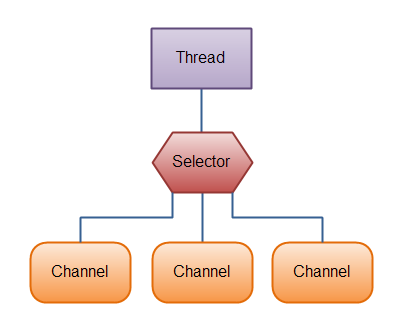
\includegraphics[scale=0.65]{./Figs/selectors.png}
  \caption
  {A thread using Selector to handle 3 Channels}
  \label{FigSelector}
\end{figure}

\paragraph*{Packet Structure} The packet sent between the clients needs to contain information about all aspect of the game. This includes player creation, action, acknowledgement, error handling as well as action sequencing. Code \ref{CodeMazewarPacket} shows the proposed packet structure. 

{
\singlespacing
\begin{lstlisting}[caption = {[MazewarPacket.java]Structure of packets exchanged between players}, label = CodeMazewarPacket]
public class MazewarPacket implements Serializable {
    public static final int NULL = 0;
    public static final int ERROR_DUPLICATED_CLIENT = 1;
    public static final int ERROR_DUPLICATED_LOCATION = 1;

    public static final int REGISTER = 100;
    public static final int REGISTER_SUCCESS = 101;

    public static final int ADD = 103;
    public static final int ADD_SUCCESS = 104;

    public static final int MOVE_FORWARD = 105;
    public static final int MOVE_BACKWARD = 106;

    public static final int TURN_LEFT = 206;
    public static final int TURN_RIGHT = 207;

    public static final int FIRE = 300;
    public static final int KILLED = 301;

    public static final int FIRST = 400;
    public static final int PROPOSE = 401;
    public static final int FINAL = 402;

    public static final int QUIT = 400;

    //packet origin identifier
    public String owner;
    public String killed;

	//packet content
    public int type = MazewarPacket.NULL;
    public HashMap<String, DirectedPoint> mazeMap = 
    						new HashMap<String, DirectedPoint>();
    public HashMap<String, Integer> mazeScore = 
    						new HashMap<String, Integer>();
    public HashMap<String, Integer> mazeSequence = 
    						new HashMap<String, Integer>();
}
\end{lstlisting}
}

The packet origin identifier identifies the client who generated the packet, and in the case where two clients are involved (eg. killing), the source and target of the clients. Packet contents contains a type variable that identify the action the packet aims to perform, such as moving or turning. MazeMap variable are used to supply clients with a new location of a particular player in case of respawn or new player join. MazeScore variable is used to update new joined player with current score table. MazeSequence is used to maintain a total order of packet deliver accorss, the detail of this design is presented in Section \ref{DesignConsistency}.

\subsection{How a player Locate, Leave and Join}\label{DesignGameFlow}

This section puts all the component together to describe the life cycle of the game play. First of all, when a player wishes to join the game, a query is sent to the naming service which replies with a list of currently connected player, and the socket address they are listening on. The new player then establishes connection with all provided sockets, and wait for the other players to acknowledge this join request. When the existing player receives a new player request, it register the new connection locally, and replies with its own current location. After the new player have received reply from everyone else it then starts to process any action related packet in the hold-back queue based on sequence number.

When a player decides to leave, it sends a broadcast packet with type QUIT as in Code \ref{CodeMazewarPacket}, and waits for acknowledgement from all players. When all the players acknowledge the quit, the player can then gracefully exit. This is to maintain total order as described in Section \ref{DesignConsistency}.

\subsection{Maintaining Consistency}\label{DesignConsistency}

Consistency is a major issue in a distributed game in this case. To demonstrate possible scenario of inconsistent state, we will look at several cases. First of all, consider player A and player B both made a move to position (12,7). Player B will see its own movement first and the broadcast packet from player A second, and declare that player B has arrived at (12,7) first. Similarly player A will think itself arrived first, resulting in two different game state. Second of all, we look at two players that are right next to each other firing at each other at the same time. This is quite a frequent scenario since there are many corners that leads to players facing each other. Similar to the first case, the local players might see different order of event resulting in differnt player being vaporized on different machine. Thirdly, when a new player joins dynamically, it must captures the current game state, and put all subsequence movement on hold before the current game state and be processed and displayed. This again requires an ordering of event accross the game.

To solve this issue, we realized that an ordering needs to be established. Several types of ordering in a distributed system were looked at. First, the FIFO ordering only guarantees that if process A produces a happens-before relation, then this relation is captured on all other processes broadcasted to, it provides no information on order accorss processes. Secondly, the Causual ordering were looked at, which guarantees if message m -$>$ m' where -$>$ is the happened-before relation induced, then any other process will also deliver m before m'. This again does not guarantee two process will have same order of execution. Finially we arrive at total ordering, which guarantees that the order of execution will be maintained throughout the system.

Total ordering leads to a consistent game state at all times accross all players, and should be applied as part of this design. We should note that total ordering does not guarantee fairness in real time. For example, if player A and B are next to each other and fires at one another, if player A fired first, and player B second, total ordering does not guarantee that player A will always kill player B. Instead, it guarantees that if player B killed player A, everyone in the game will see the same state. To achieve total fairness, a phyical clock synchronization is needed.
